\documentclass{ximera}
\usepackage{sagetex}
%% handout
%% space
%% newpage
%% numbers
%% nooutcomes

%% You can put user macros here
%% However, you cannot make new environments

\graphicspath{{./}{module1Activity/}{module2Activity/}{module3Activity/}}

\usepackage{sagetex}
\usepackage{tikz}
\usepackage{hyperref}
\usepackage{tkz-euclide}
\usetkzobj{all}
\pgfplotsset{compat=1.7} % prevents compile error.

\tikzstyle geometryDiagrams=[ultra thick,color=blue!50!black]
 %% we can turn off input when making a master document

\outcome{}
\author{Darryl Chamberlain Jr.}

\title{Objective 3 - Evaluating Limits}

\begin{document}
\begin{abstract}
Interpret the notation for limits.
\end{abstract}
\maketitle

\href{https://cnx.org/contents/i4nRcikn@5.1:dKCfyV9u@5/The-Limit-of-a-Function}{Link to section in online textbook.}

\href{https://www.youtube.com/watch?v=riXcZT2ICjA}{Video for evaluating a limit.}

%%%%%%%%%%%%%%%%%%%%%
%%%  Objective 3  %%%
%%%%%%%%%%%%%%%%%%%%%

Now that we have learned about left- and right-hand limits, we can evaluate the limit of a function at a point.

\begin{theorem}
	Evaluating the limit of a function at a point $x=a$:
	\begin{center}

		$\lim_{x \rightarrow a} (f(x)) = L$

		if and only if

		$\lim_{x \rightarrow a^{-}} (f(x)) = L = \lim_{x \rightarrow a^{+}} (f(x))$
	\end{center}

	Note: The limit \textbf{exists} if $L$ is a Real number. The limit can be equal to $\infty$ or $-\infty$, but we would not say that it exists. If the left- and right-hand limits do not agree, we say \textbf{the limit does not exist} (or DNE for short).
\end{theorem}

This objective will allow you to practice evaluating the left- and right-hand limits to determine if the limit at a point exists. \textbf{This would be where you want to practice before the exam.}

\textbf{Answers are either a Real number, $\infty$, $-\infty$, or DNE.}

% GRAPH
\begin{question}
\begin{figure}
	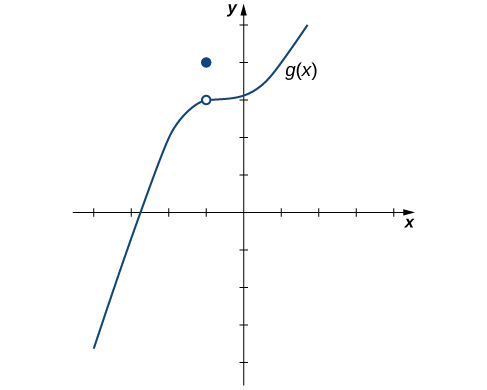
\includegraphics{CNX_Calc_Figure_02_02_006.jpg}
	\caption{\href{https://cnx.org/contents/i4nRcikn@5.1:dKCfyV9u@5/The-Limit-of-a-Function\#CNX_Calc_Figure_02_02_006}{Function with a hole at $x=-1$.}}
\end{figure}

$\lim_{x \rightarrow -\infty} f(x) = \answer{\sage{-Infinity}}$

$\lim_{x \rightarrow -1} g(x) = \answer{3}$

$\lim_{x \rightarrow \infty} f(x) = \answer{\sage{Infinity}}$

\end{question}

% GRAPH
\begin{question}
\begin{figure}
	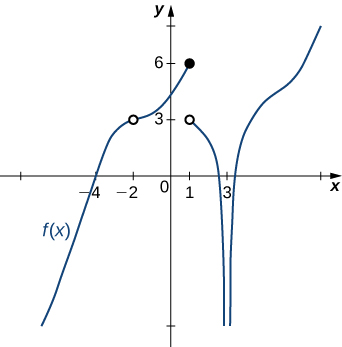
\includegraphics{CNX_Calc_Figure_02_02_015.jpg}
	\caption{\href{https://cnx.org/contents/i4nRcikn@5.1:dKCfyV9u@5/The-Limit-of-a-Function\#CNX_Calc_Figure_02_02_015}{Piecewise function to evaluate.}}
\end{figure}

$\lim_{x \rightarrow -\infty} f(x) = \answer{\sage{-Infinity}}$

$\lim_{x \rightarrow -2} f(x) = \answer{3}$

$\lim_{x \rightarrow 1} f(x) = \answer[format=string]{DNE}$

$\lim_{x \rightarrow 3} f(x) = \answer{\sage{-Infinity}}$

$\lim_{x \rightarrow \infty} f(x) = \answer{\sage{Infinity}}$

\end{question}

% GRAPH
\begin{question}
\begin{figure}
	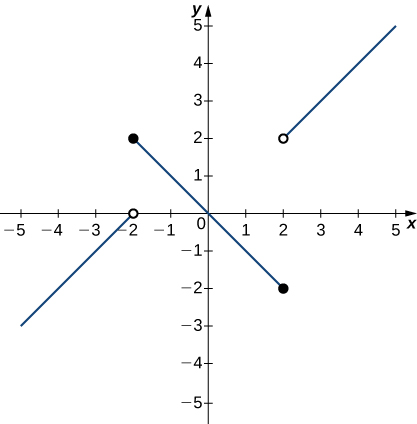
\includegraphics{CNX_Calc_Figure_02_02_204.jpg}
	\caption{\href{https://cnx.org/contents/i4nRcikn@5.1:dKCfyV9u@5/The-Limit-of-a-Function\#CNX_Calc_Figure_02_02_204}{Piecewise function to evaluate.}}
\end{figure}

$\lim_{x \rightarrow -\infty} f(x) = \answer{\sage{-Infinity}}$

$\lim_{x \rightarrow -2} f(x) = \answer[format=string]{DNE}$

$\lim_{x \rightarrow 0} f(x) = \answer{0}$

$\lim_{x \rightarrow 2} f(x) = \answer[format=string]{DNE}$

$\lim_{x \rightarrow \infty} f(x) = \answer{\sage{Infinity}}$

\end{question}

% GRAPH
\begin{question}
\begin{figure}
	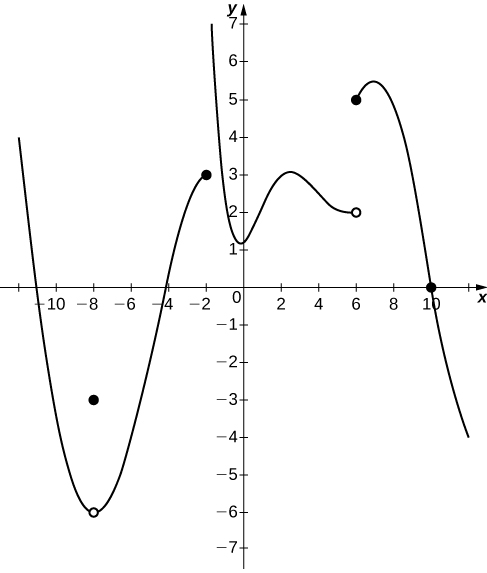
\includegraphics{CNX_Calc_Figure_02_02_201.jpg}
	\caption{\href{https://cnx.org/contents/i4nRcikn@5.1:dKCfyV9u@5/The-Limit-of-a-Function\#CNX_Calc_Figure_02_02_201}{Piecewise function to evaluate.}}
\end{figure}

$\lim_{x \rightarrow -\infty} f(x) = \answer{\sage{Infinity}}$

$\lim_{x \rightarrow -8} f(x) = \answer{-6}$

$\lim_{x \rightarrow -2} f(x) = \answer[format=string]{DNE}$

$\lim_{x \rightarrow 6} f(x) = \answer[format=string]{DNE}$

$\lim_{x \rightarrow 10} f(x) = \answer{0}$

$\lim_{x \rightarrow \infty} f(x) = \answer{\sage{-Infinity}}$

\end{question}

% Analytical - Hole
\begin{sagesilent}
factor5A = ZZ.random_element(2, 5)*x - ZZ.random_element(2, 5)*(-1)**ZZ.random_element(2)
factor5B = ZZ.random_element(2, 5)*x - ZZ.random_element(2, 5)*(-1)**ZZ.random_element(2)
value5A = solve(factor5A == 0, x)[0].rhs()
value5B = solve(factor5B == 0, x)[0].rhs()
while value5A == value5B:
    factor5A = ZZ.random_element(2, 5)*x - ZZ.random_element(2, 5)*(-1)**ZZ.random_element(2)
    factor5B = ZZ.random_element(2, 5)*x - ZZ.random_element(2, 5)*(-1)**ZZ.random_element(2)
    value5A = solve(factor5A == 0, x)[0].rhs()
    value5B = solve(factor5B == 0, x)[0].rhs()
numeratorOnDisplay5 = factor5A*factor5B
disguiseDenominator5 = (-1)**ZZ.random_element(2) * ZZ.random_element(2, 5)
denominatorOnDisplay5 = disguiseDenominator5 * factor5A
function5 = numeratorOnDisplay5/denominatorOnDisplay5
#
if disguiseDenominator5 > 0:
    limitAtNegInfty5 = -Infinity
    limitAtInfty5 = Infinity
else:
    limitAtNegInfty5 = Infinity
    limitAtInfty5 = -Infinity
#
limitAtValue5A = factor5B(x = value5A) / disguiseDenominator5
limitAtValue5B = 0
\end{sagesilent}

\begin{question}
$ f(x) = \frac{\sage{numeratorOnDisplay5}}{\sage{denominatorOnDisplay5}}$

$\lim_{x \rightarrow -\infty} f(x) = \answer{\sage{limitAtNegInfty5}}$

$\lim_{x \rightarrow \sage{value5A} } f(x) = \answer[tolerance=0.01]{\sage{limitAtValue5A}}$

$\lim_{x \rightarrow \sage{value5B} } f(x) = \answer[tolerance=0.01]{\sage{limitAtValue5B}}$

$\lim_{x \rightarrow \infty} f(x) = \answer{\sage{limitAtInfty5}}$
\end{question}

% Analytical - VA and Hole
\begin{sagesilent}
factor6A = ZZ.random_element(2, 5)*x - ZZ.random_element(2, 5)*(-1)**ZZ.random_element(2)
factor6B = ZZ.random_element(2, 5)*x - ZZ.random_element(2, 5)*(-1)**ZZ.random_element(2)
value6A = solve(factor6A == 0, x)[0].rhs()
value6B = solve(factor6B == 0, x)[0].rhs()
while value6A == value6B:
    factor6A = ZZ.random_element(2, 5)*x - ZZ.random_element(2, 5)*(-1)**ZZ.random_element(2)
    factor6B = ZZ.random_element(2, 5)*x - ZZ.random_element(2, 5)*(-1)**ZZ.random_element(2)
    value6A = solve(factor6A == 0, x)[0].rhs()
    value6B = solve(factor6B == 0, x)[0].rhs()
numeratorOnDisplay6 = factor6B
disguiseDenominator6 = (-1)**ZZ.random_element(2) * ZZ.random_element(2, 5)
denominatorOnDisplay6 = disguiseDenominator6 * factor6A * factor6B
function6 = numeratorOnDisplay6/denominatorOnDisplay6
#
limitAtNegInfty6 = 0
limitAtInfty6 = 0
#
limitAtValue6A = "DNE"
limitAtValue6B = 1/(disguiseDenominator6 * factor6A(x = value6B))
\end{sagesilent}

\begin{question}
	$ f(x) = \frac{\sage{numeratorOnDisplay6}}{\sage{denominatorOnDisplay6}}$

	$\lim_{x \rightarrow -\infty} f(x) = \answer{\sage{limitAtNegInfty6}}$

	$\lim_{x \rightarrow \sage{value6A} } f(x) = \answer[format=string]{DNE}$

	$\lim_{x \rightarrow \sage{value6B} } f(x) = \answer[tolerance=0.01]{\sage{limitAtValue6B}}$

	$\lim_{x \rightarrow \infty} f(x) = \answer{\sage{limitAtInfty6}}$
\end{question}

\begin{sagesilent}
# Equation: $\lim_{x \rightarrow 0} (ax+1)^(1/x) = e^a$
a6 = ZZ.random_element(1, 5)
equation6 = (a6*x + 1)**(1/x)
limitAtEquation6 = [0, equation6, exp(a6)]
\end{sagesilent}
\begin{question}
$ \lim_{x \rightarrow \sage{limitAtEquation6[0]}} \sage{limitAtEquation6[1]} = \answer[tolerance=0.01]{\sage{limitAtEquation6[2]}}$

\begin{hint}
We can't plug in the exact value, so we will need to plug in values very near $\sage{limitAtEquation6[0]}$.
\end{hint}
\end{question}

\begin{sagesilent}
# Equation: $lim_{x \rightarrow eqA} \frac{\sqrt{x-eqC} - eqB}{x-eqA}$
eqB = ZZ.random_element(2, 6)
eqC = ZZ.random_element(1, 5)
eqA = eqB**2 + eqC
limitAtEquation7 = 1/(2*eqB)
\end{sagesilent}
\begin{question}
$ \lim_{x \rightarrow \sage{eqA}} \frac{ \sqrt{ x - \sage{eqC} } - \sage{eqB}}{ x - \sage{eqA} } = \answer[tolerance=0.01]{\sage{limitAtEquation7}}$

\begin{hint}
We can't plug in the exact value, so we will need to plug in values very near $\sage{eqA}$.
\end{hint}
\end{question}

\end{document}
